\section{UV-VIS Spectroscopy}
\label{sec:uv-vis}

\subsection{Influence of the solvent}

In the following, the UV/VIS spectra of ZnTPP dissolved in toluene and benzonitrile are compared. A spectral shift is noticeable, the peak for toluene is at shorter wavelengths than that for benzonitrile.
\begin{center}
    \captionsetup{type = figure}
    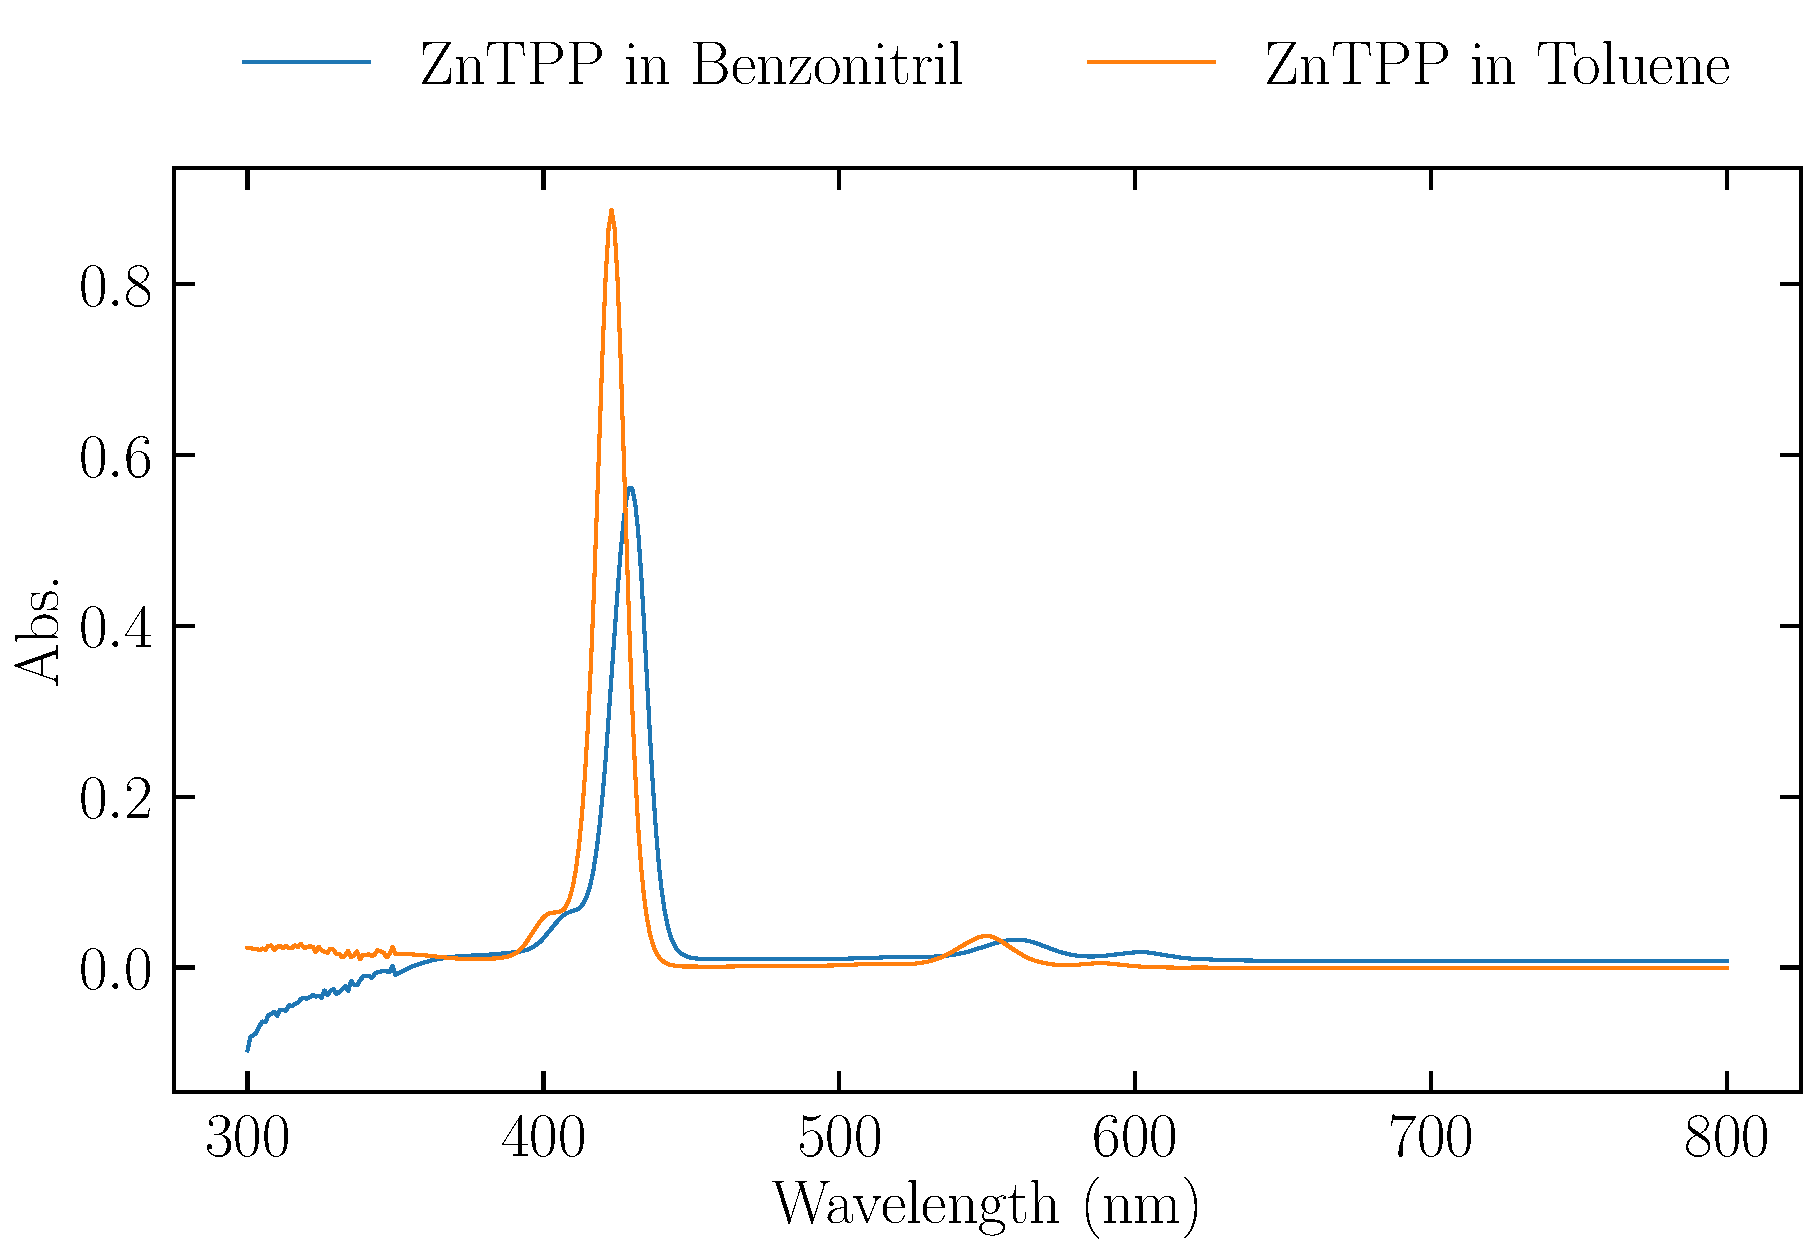
\includegraphics[width = 0.85\textwidth]{Pictures/Evaluation/41/ZnTpp-in-Bn-Tol.pdf}
    \captionof{figure}{
        UV/VIS absorbance spectrum of ZnTPP in benzonitril and toluene.
    }
    \label{fig:uv-visBNTol}
\end{center}
One possible cause is the reorganization of the solvent molecules around the target molecule as it transitions from the ground state to the excited state, leading to changes in symmetry and charge distribution, depending on the solvent.

In addition, the solvent itself can influence the confirmation of the dissolved molecules, which can also cause such an energy difference.


\subsection{Comparison of zinc complexes}

In the following, the absorption spectra of the zinc complexes will be compared. Before this is pursued further, it should be noted that the absorption spectrum of ZnTPP is in good qualitative agreement with the literature \citep{Nojiri.1998}.

\begin{center}
    \captionsetup{type = figure}
    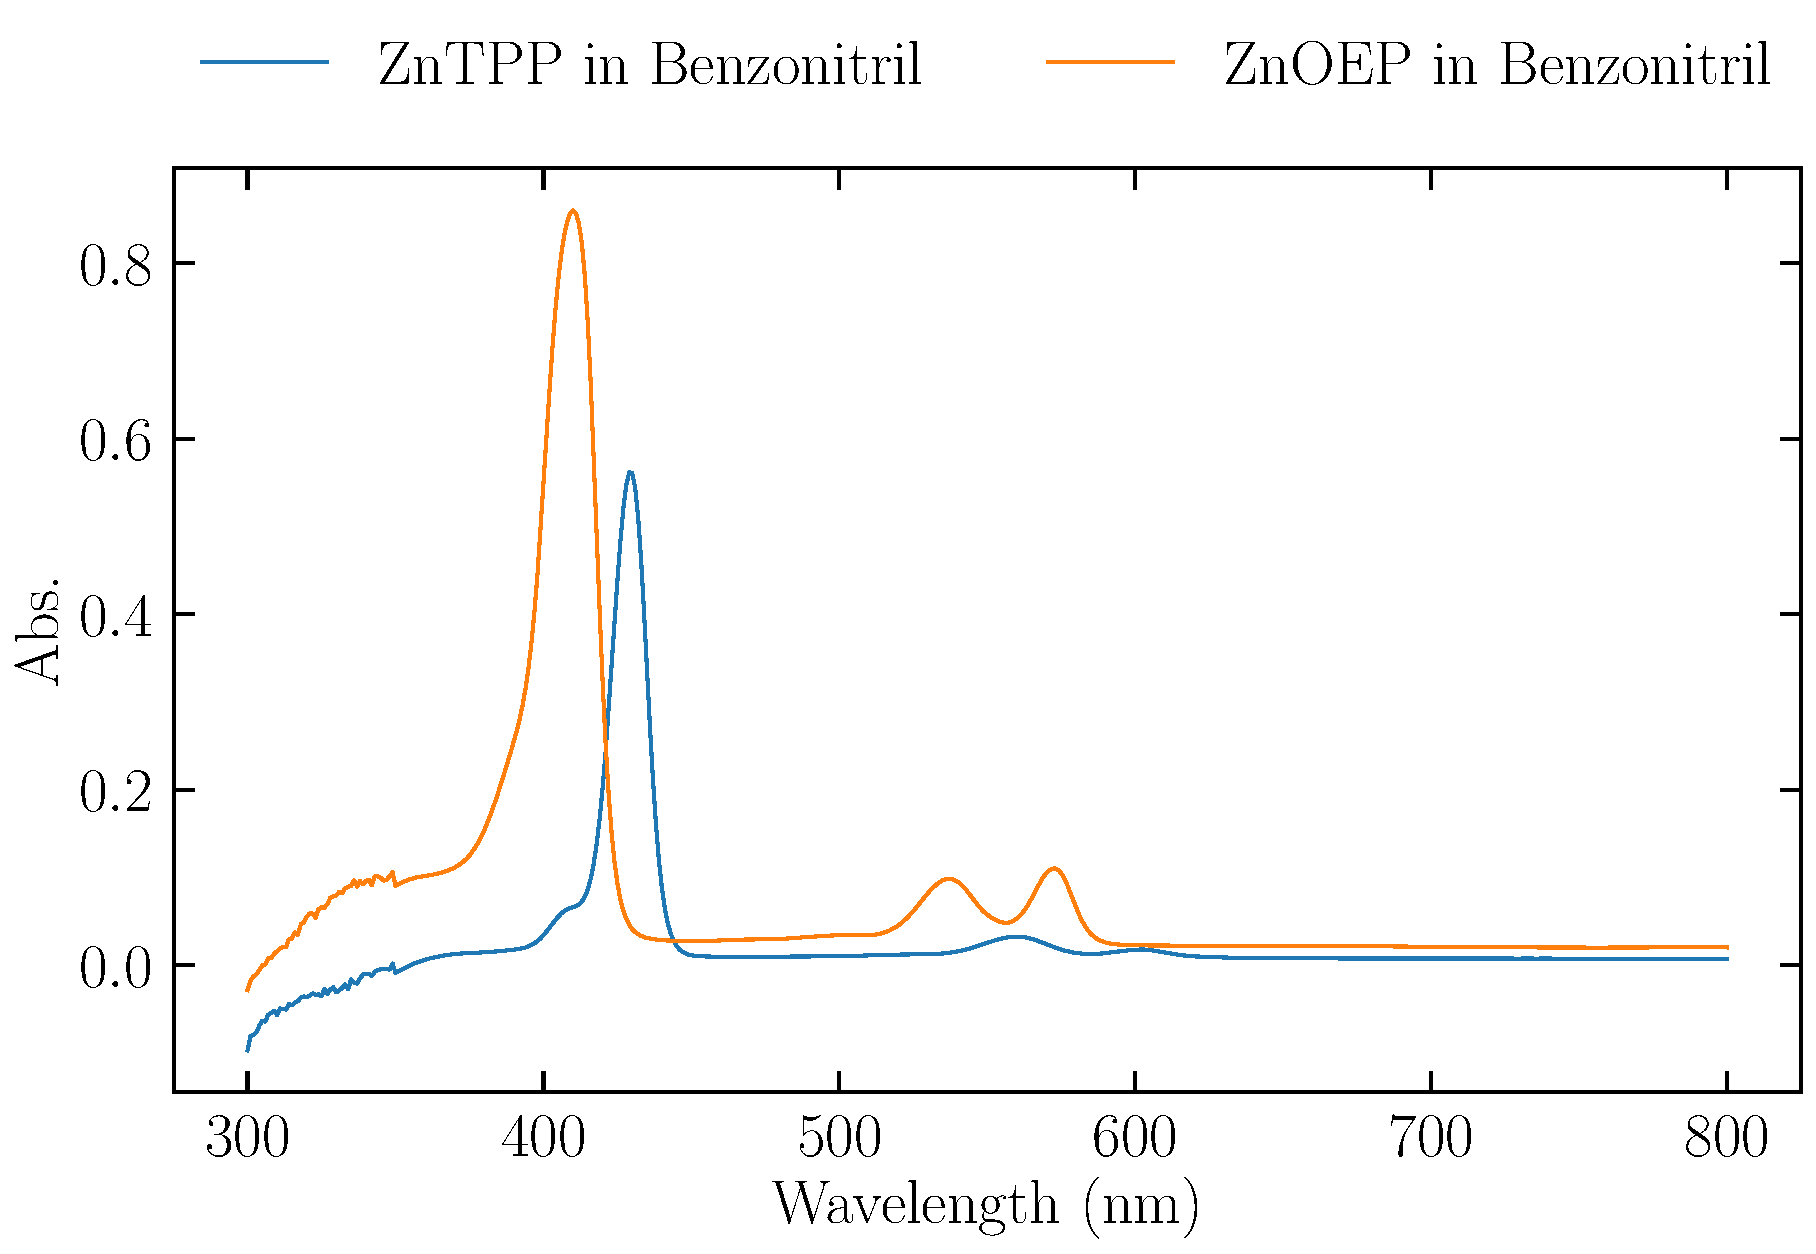
\includegraphics[width = 0.85\textwidth]{Pictures/Evaluation/41/ZnTpp-ZnOEP-in-Bn.pdf}
    \captionof{figure}{
        UV/VIS absorbance spectrum of ZnTPP and ZnOEP in benzonitril.
    }
    \label{fig:uv-visZinc}
\end{center}

It can be clearly seen that the main work of ZnOEP is at higher energies than that of ZnTPP. Which can probably be explained by the structure. In contrast to ZnOEP, ZnTPP has four benzene rings. These extend the system of conjugated $\pi$-bonds, which leads to a reduction in absorption energy.
